\documentclass{amsart}
\usepackage{style/preamble}
\usepackage{parskip}
\begin{document}
\section*{Classification of surfaces}

\begin{theorem}
  Every compact Riemann surface is homeomorphic(=topologically isomorphic) to a surface of genus $g$.
  \begin{figure}[H]
    \centering 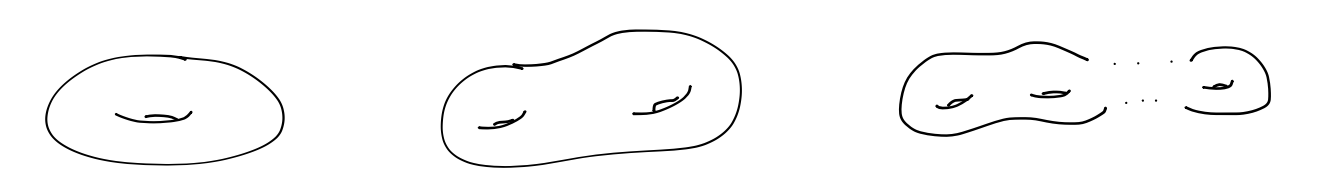
\includegraphics[width=0.85\linewidth]{images/GegusGSurfaces}
    \caption{Torus, genus 2 surface, higher genus surfaces}
  \end{figure}
  Upto isomorphism, there is exactly one Riemann surface of genus 0, namely the Riemann sphere $\bbp^1$.
\end{theorem}

The genus can be thought of as the number of ``handles'' in the surface.

\textbf{Word of caution:} Two Riemann surfaces being homeomorphic does not mean that they are isomorphic as Riemann surfaces.
We will show that every elliptic curve is homeomorphic to the genus 1 surface (=torus) but not all elliptic curves are isomorphic to each other as Riemann surfaces.








\section*{Euler characteristic}
  It is possible to compute the genus using triangulations of surfaces.
  For any triangulation of a genus $g$ surface $M$ with $V$ vertices, $E$ edges, and $F$ faces, we have the following identity:
  \begin{align*}
    2 - 2g = V - E + F.
  \end{align*}
  The important point here is that the right-hand side depends on the triangulation but the left-hand side does not. The right-hand is called the Euler characteristic of $M$, denoted $\chi(M)$.

  \begin{figure}[H]
  \centering
    % \includegraphics[width=0.5\textwidth]{example-image}
    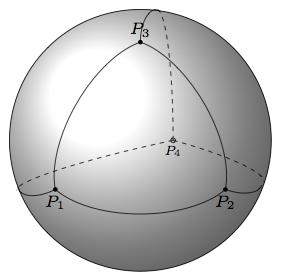
\includegraphics[width=0.45\textwidth]{images/SphereTriangulation.jpg}
    \caption{Triangulation of $S^2$ (genus=0) with $V = 4$, $E=6$, and $F = 4$ so that $V - E + F = 2 = 2 - 2 \cdot 0$.}
  \end{figure}






  \section*{Coverings of simply-connected spaces}

  A topological space $Y$ is said to be \emph{simply-connected} if it is connected and every loop in $Y$ can be continuously contracted to a point.

  \begin{figure}[H]
  \centering
    % \includegraphics[width=0.5\textwidth]{example-image}
    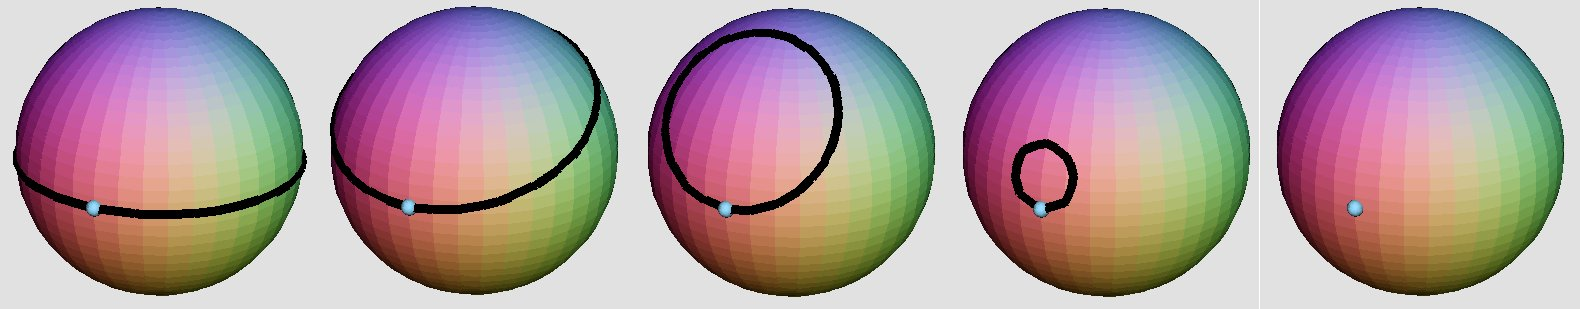
\includegraphics[width=0.9\textwidth]{images/S2isSimplyConnected.jpg}
  \end{figure}


  For example, the Riemann sphere $\bbp^1$ is simply-connected. If we remove a single point or a single path-connected set from $\bbp^1$, the resulting space is still simply-connected.

  But if $Y$ is the space obtained by removing two or more points from the Riemann sphere, then $Y$ is not simply-connected.

  This is the only example that concerns us.

  \begin{theorem}
    If $f: X \rightarrow Y$ is a continuous $n:1$ (covering) map and $Y$ is simply-connected then $X$ is topologically isomorphic to $n$ disjoint copies of $Y$.
  \end{theorem}
  For this theorem we do not allow any ramification points, so $f$ needs to a genuine $n:1$ (covering) map.







\end{document}
